	Mediante la herramienta de análisis de Fourier provista por \texttt{SPICE Orcad} se analizó la variación de la distorsión armónica \texttt{THD} producida en la salida, en función de la frecuencia y amplitud de la señal de entrada. Los resultados obtenidos se resumen en la tabla.


\begin{figure}[H]
	\centering
	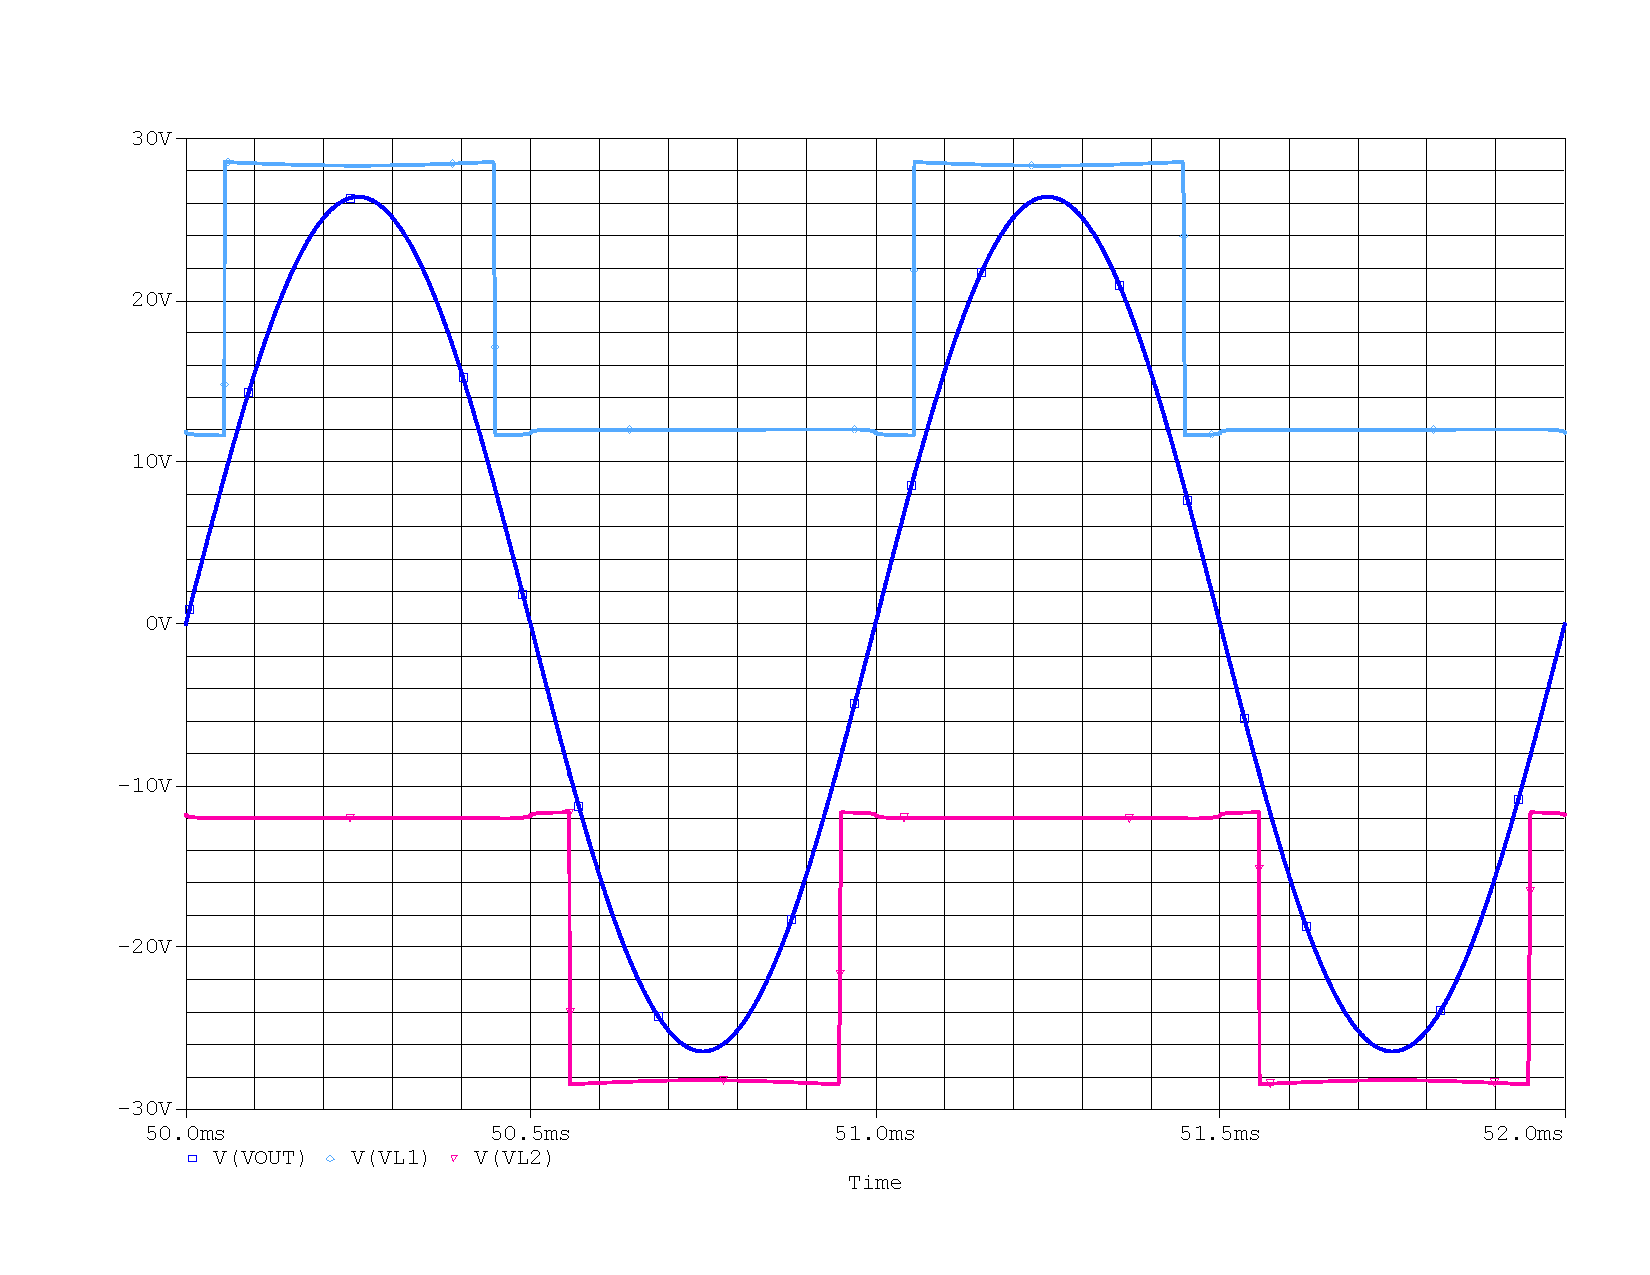
\includegraphics[scale=0.4]{sim_salida1k_max.pdf}
	\caption{Máxima excursión de salida sin recorte a \SI{1}{\kilo\hertz} $THD = 0,079\%$.}
	\label{fig:sim_salida_1k_max}
	\end{figure}

\begin{figure}[H]
	\centering
	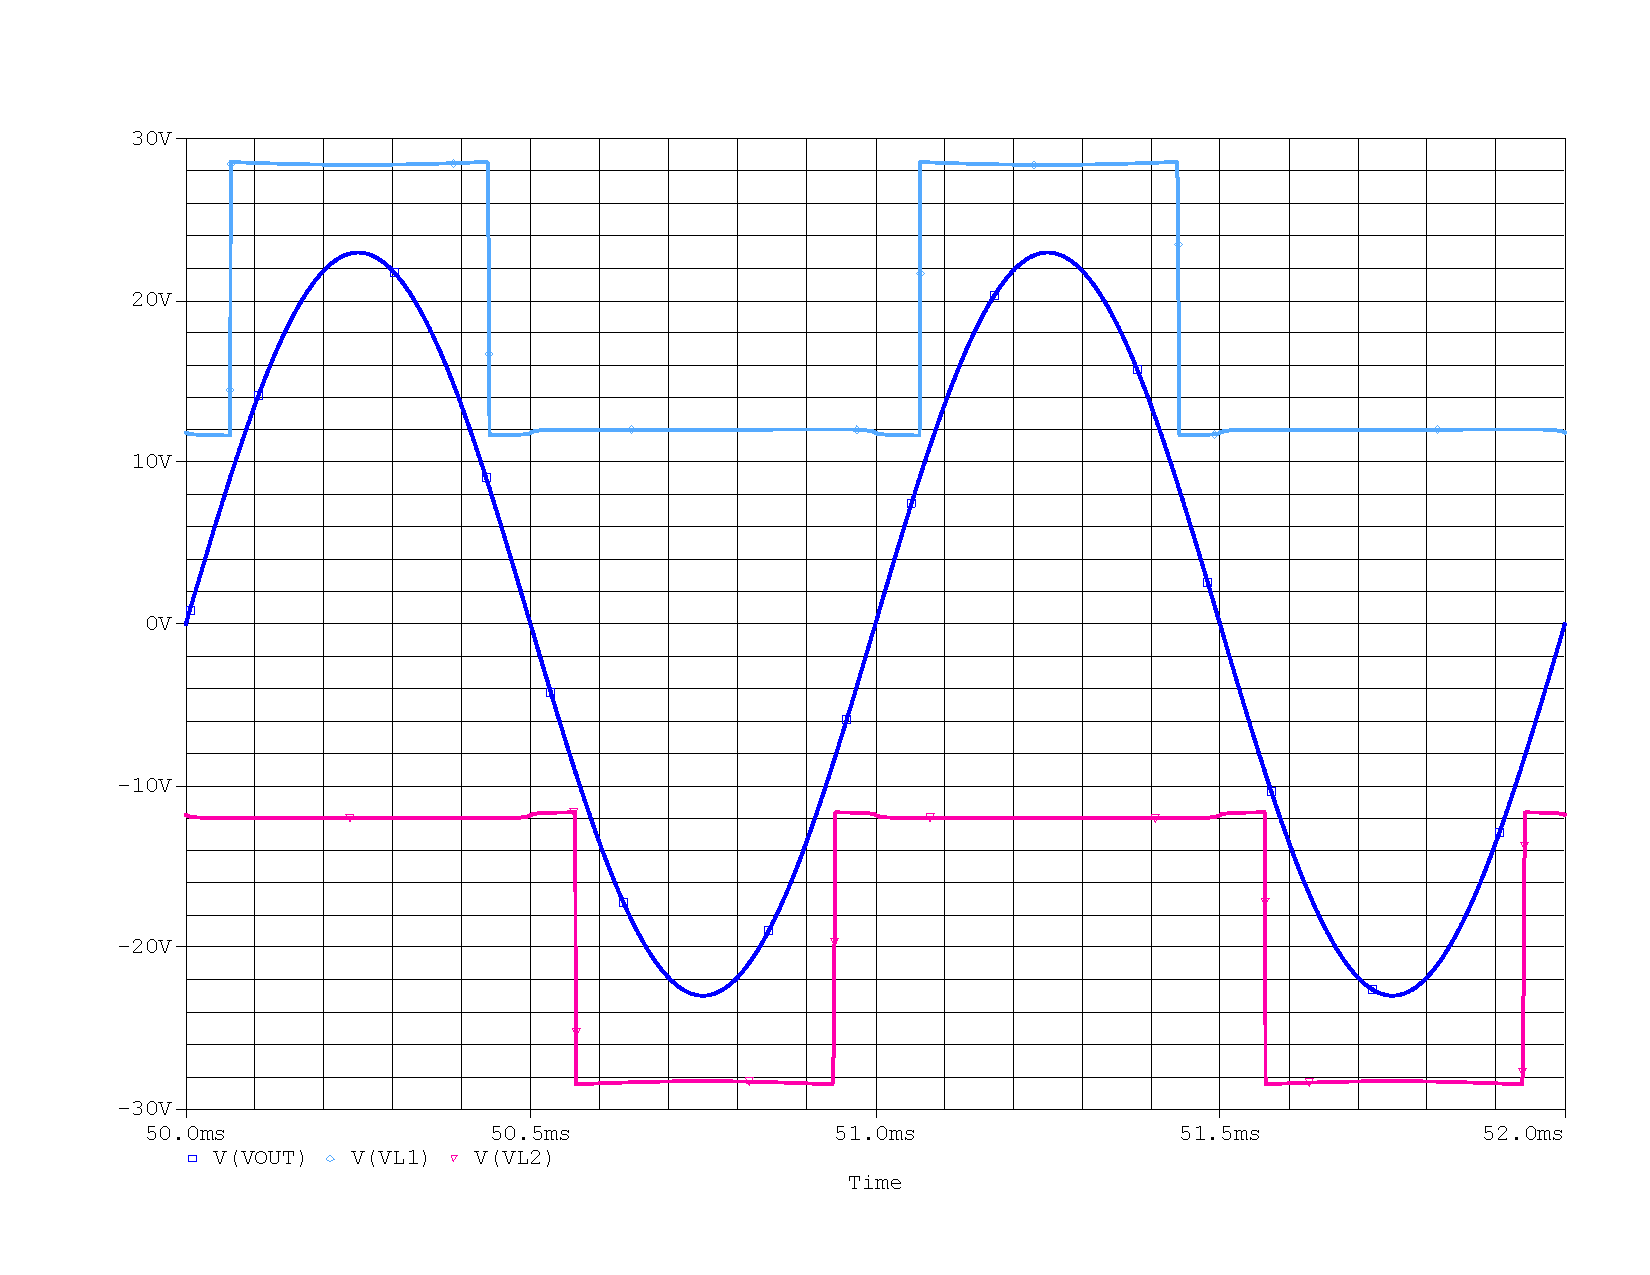
\includegraphics[scale=0.4]{sim_salida_1k_22V.pdf}
	\caption{22V, 1V, $THD=0,0976\%$.}
	\end{figure}

\begin{figure}[H]
	\centering
	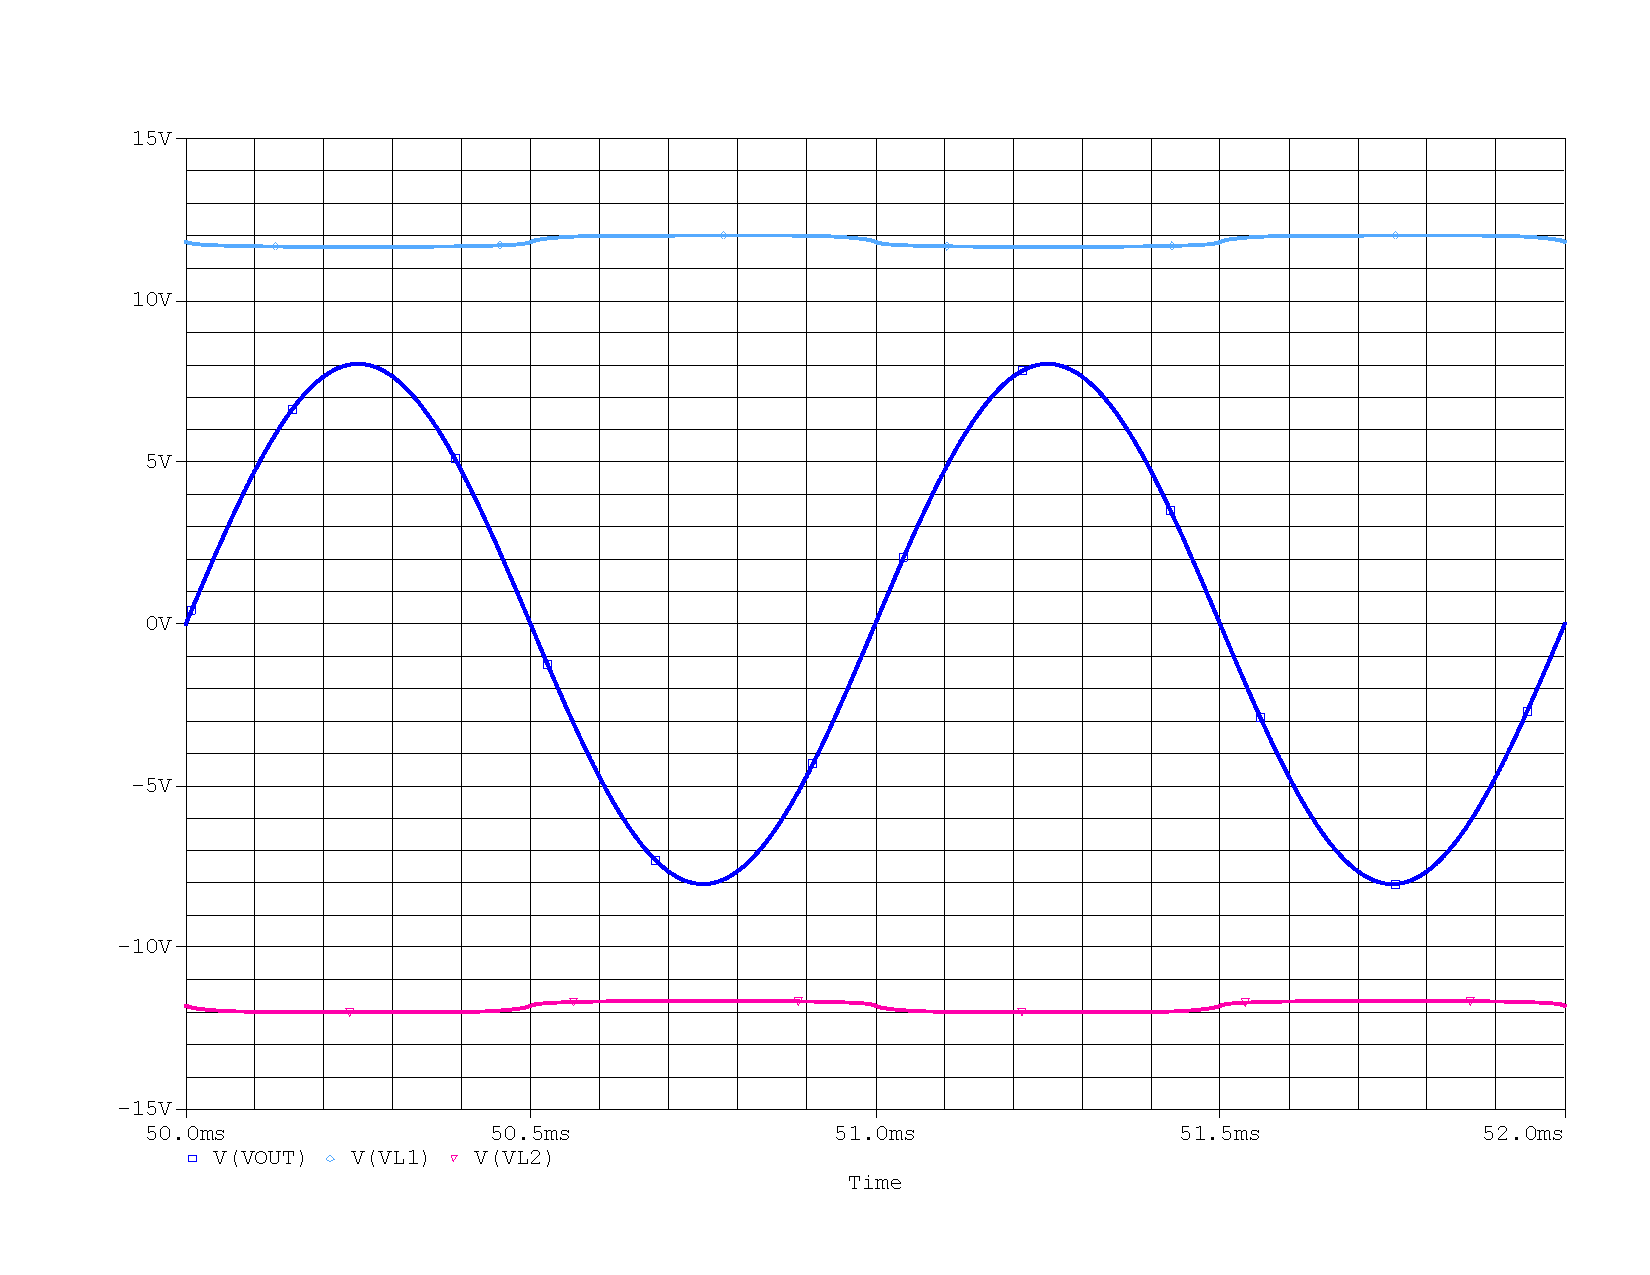
\includegraphics[scale=0.4]{sim_salida_1k_8V.pdf}
	\caption{8V, $0,35V, THD=0,061\%$.}
\end{figure}

%%%% 20kHz
\begin{figure}[H]
	\centering
	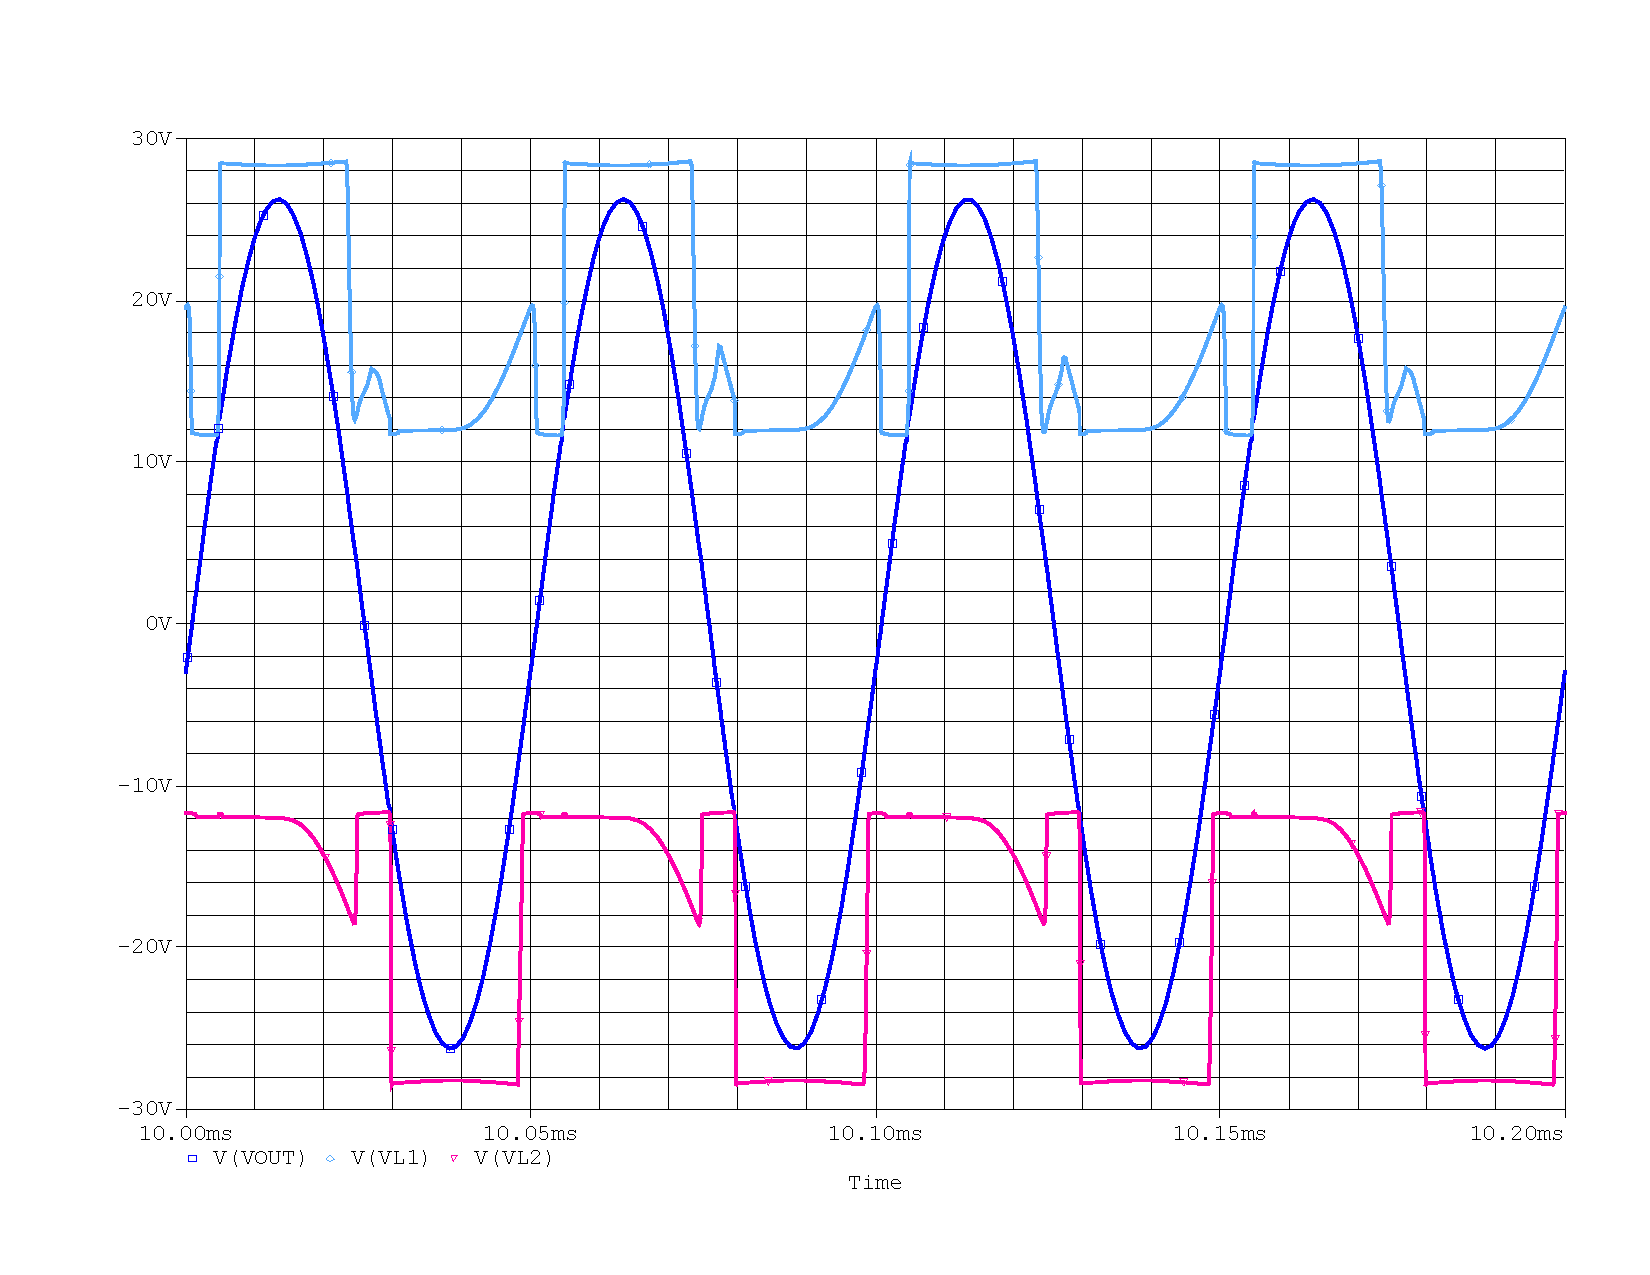
\includegraphics[scale=0.4]{sim_salida_20k_max.pdf}
	\caption{$26,1V, 0,35V, THD=0,34\%$.}
\end{figure}

\begin{figure}[H]
	\centering
	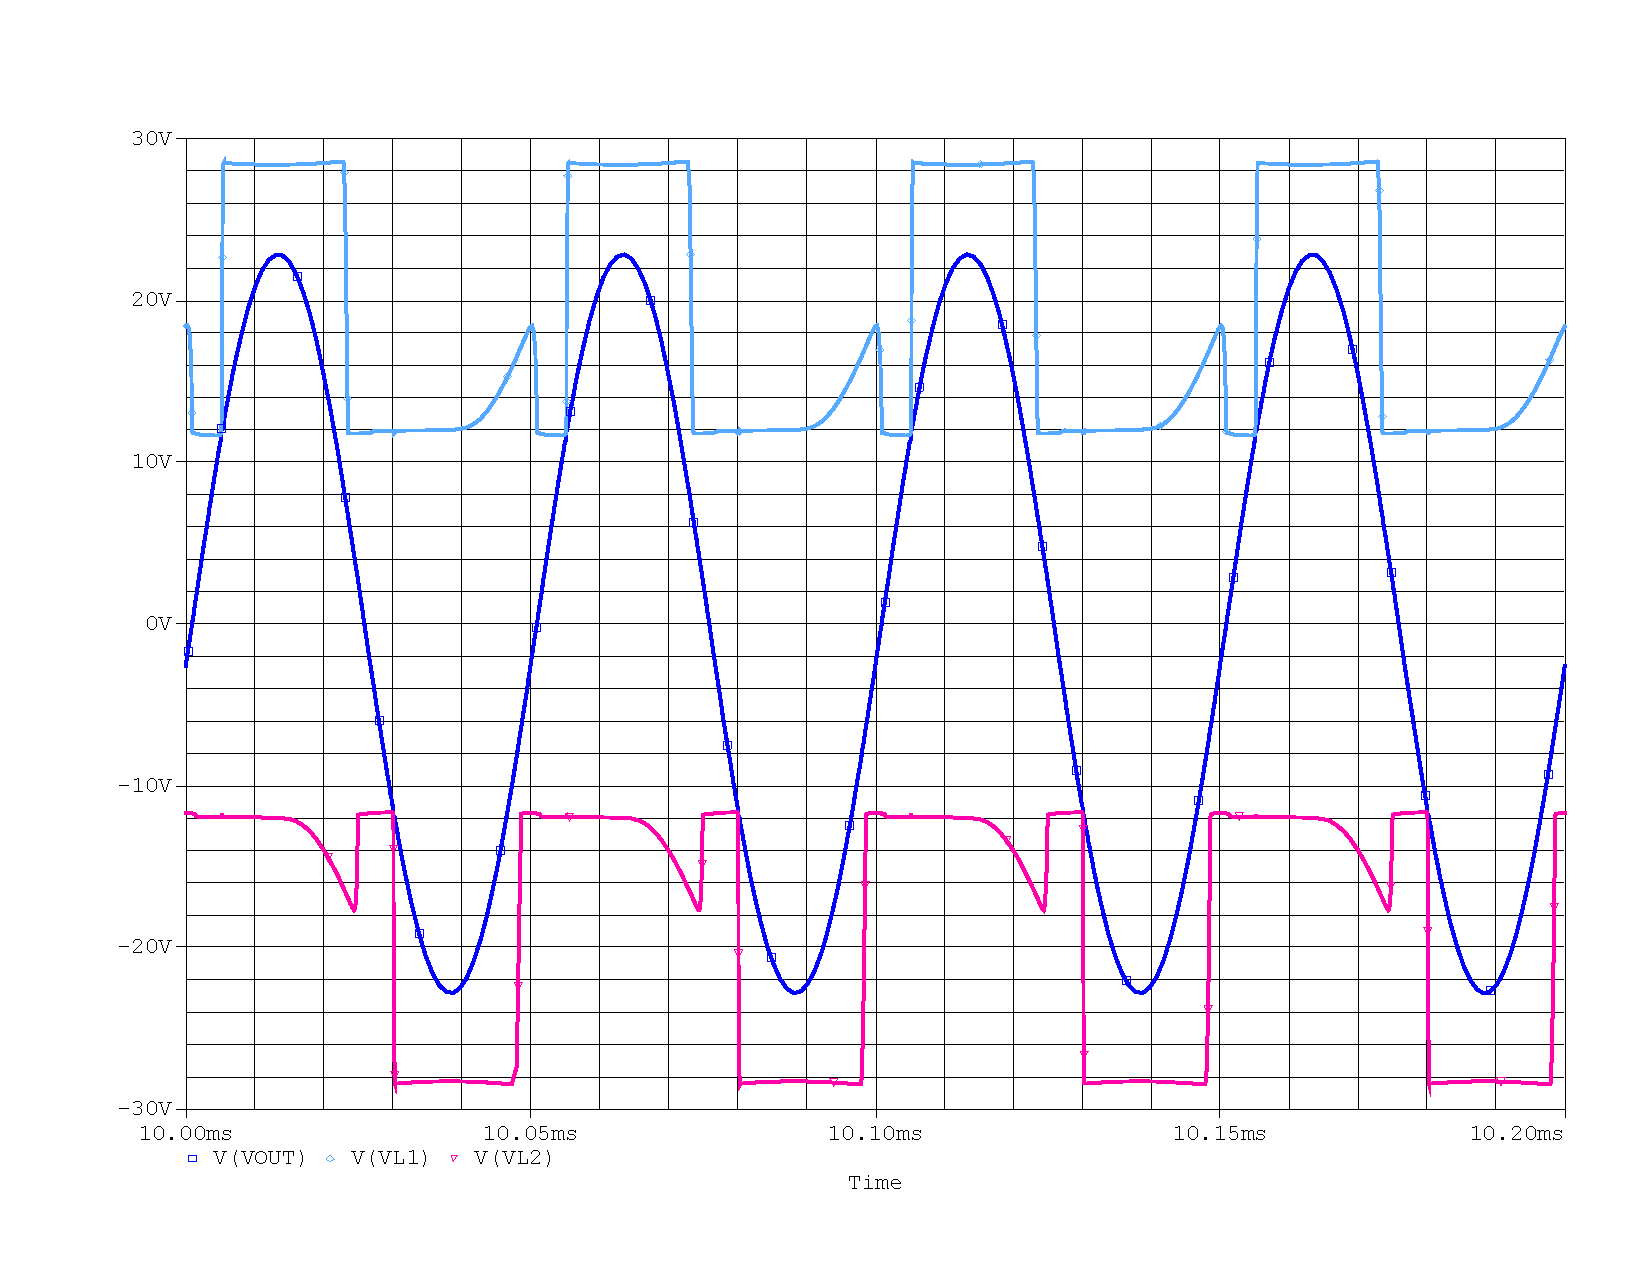
\includegraphics[scale=0.4]{sim_salida_20k_22V.pdf}
	\caption{$22V, 1V, THD=0,21\%$.}
\end{figure}

\begin{figure}[H]
	\centering
	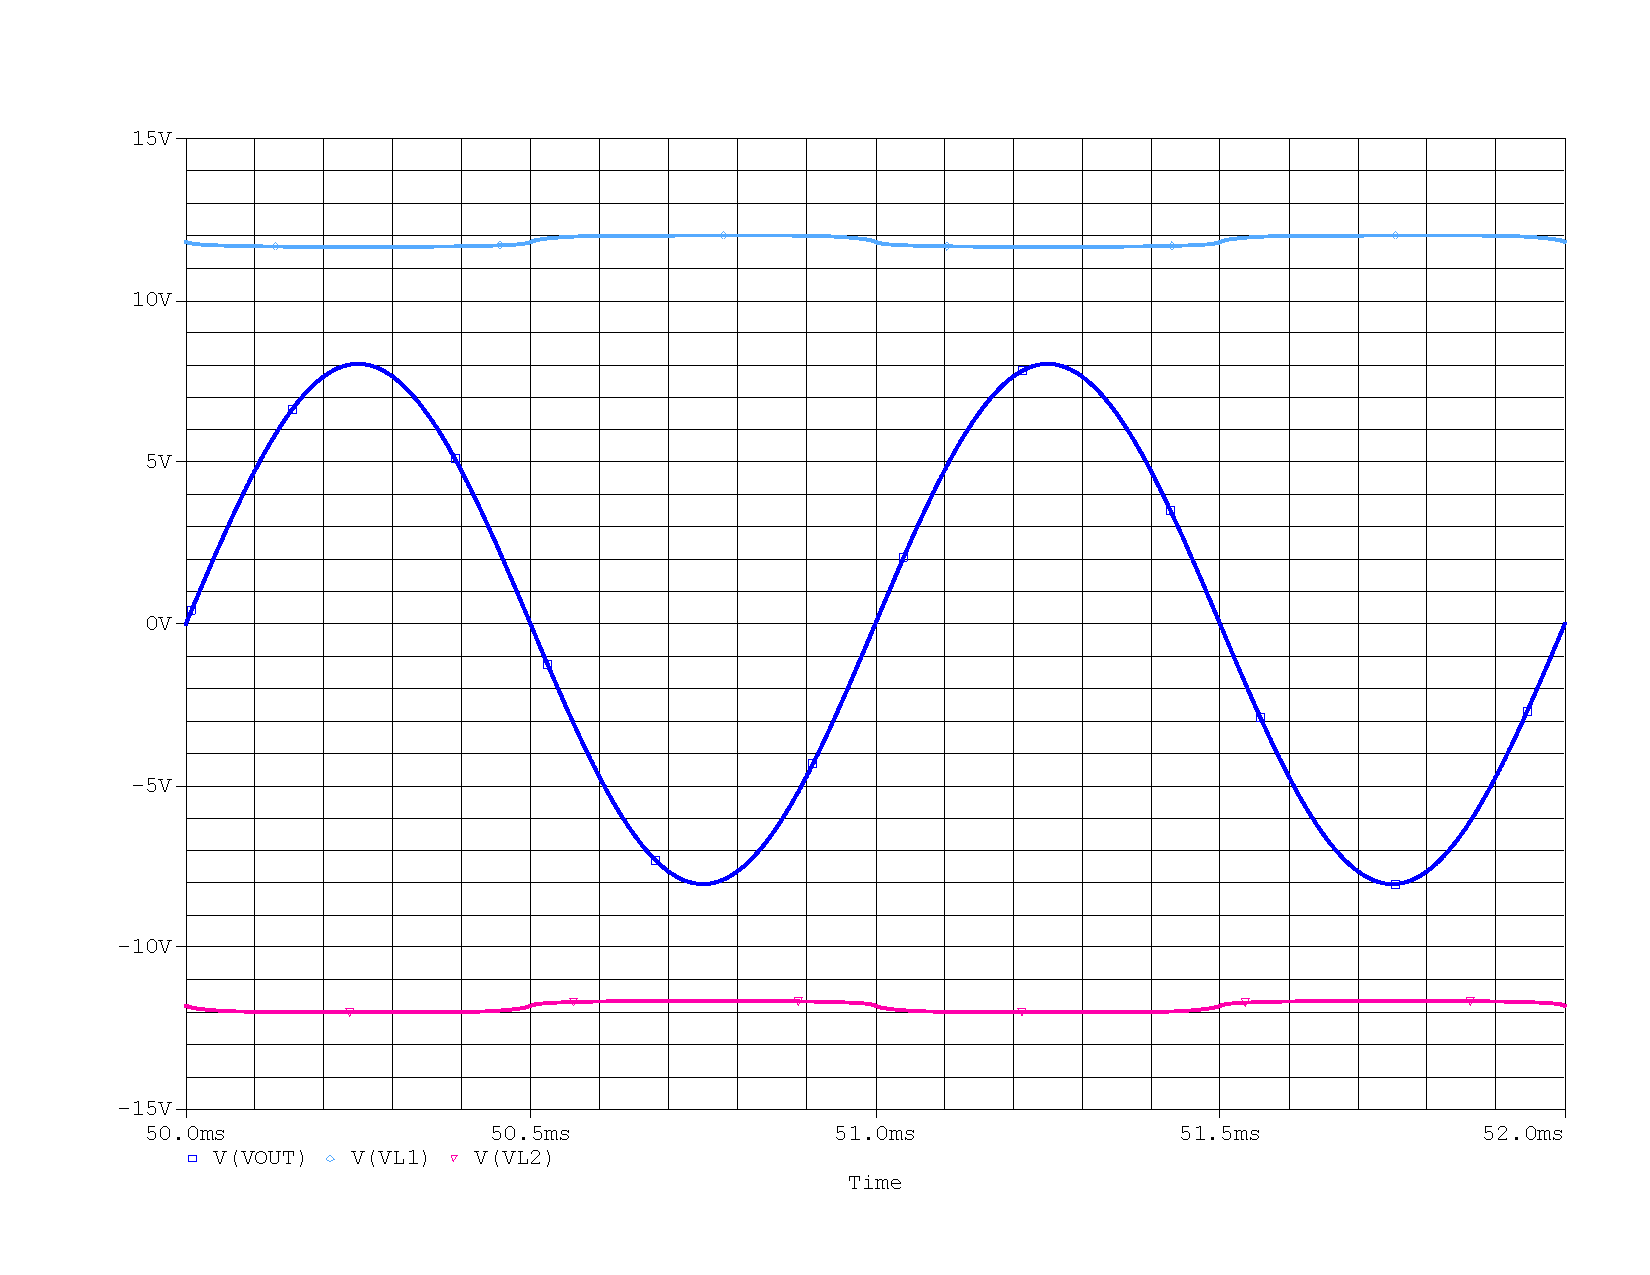
\includegraphics[scale=0.4]{sim_salida_1k_8V.pdf}
	\caption{8V, $0,35V, THD=0,23\%$.}
\end{figure}

\begin{table}[H]
	\centering
	\begin{tabular}{ccccc}
		\toprule
\multirow{2}{*}{Frecuencia} & \multicolumn{3}{c}{$P_{L,RMS}$} \\ 
		\cmidrule{2-4}
			& 4W & 30W & 42,5W \\
		\midrule
		\SI{1}{\kHz} & \num{0,061} & \num{0,0976} & \num{0,079} \\
		\SI{20}{\kHz} & \num{0.23} & \num{0,21} & \num{0,34} \\
		\bottomrule
	\end{tabular}
	\caption{Valores de $\mathrm{THD}_{\%}$ para distintos valores de frecuencia y potencias sobre la carga.}
\end{table}




